\documentclass{article}
\usepackage{hyperref}
\usepackage{pgfgantt}
\usepackage{graphicx}
\graphicspath{ {./Images/} }
\usepackage{microtype}
\begin{document}

\title{Advanced Computer Graphics}
\author{Oliver Eisenberg}
\maketitle
\twocolumn
\section{Labs}
\subsection{Lab 1 - Rasterising Lines}
The line drawing function was updated to use an interger based approach. Originally the algorithm was used for positive x,y values and then altered by mirroring the result onto the other three quadrants. This created the following image \textit{ref}. 

This seems correct, however, on further inspecution it was realised that the lines seemed to have a double thickness. This was thought to have occoured as the conditions to be in what quadrant was changing as the line was drawn. Therefore the process was reattempted in an effort to improve and refactor code.

The result was the correct output as shown here. This was done by .. . Code was refactered into a single x and y direction methods where an intial function call was responsible for determining when to call the relevant one. By calulating directions based off of the start and end coordinates.
\subsection{Lab 2 - Reading Models}
The given code in polymesh.cpp was updated to be able to read 3D objects and generate wireframes.

\subsection{Lab 3 - Simple Raytracing}
\subsubsection{Raycasting }
\subsubsection{Triangle intersection}
To compute triangle intersections the Möller–Trumbore algorithm was used. This was used instead of the method on the \textit{slides} anticipating the requirements for the baracentric coordinates to complete Gouraud shading further in the coursework.

\subsection{Lab 4 - Basic Lighting and Shadows}
Starting to work on lighting prompted further refactoring. In doing so, a scene class was created to create and store all the objectes and lighting for the render. All lights belong to the base light class, this allows to predetermine shared variables and functions a light should have.
\subsubsection{Spotlights}


\subsubsection{Pointlights}
The slides refer to two methods to create pointlights, with and without an associated direction. As spot lights are directional, pointlights with a constant intensity were implemented. This allows a pointlight to be placed between objects to cast shadow outwardss.
\subsubsection{Shadows}
Shadows are checked by sending a ray from the hit position to each light in the scene. If an intersection occours the intensity from that light is removed. This allows for shadows of different intensity depening on the source.

\section{Optimisations}
Coloured Diffuse
Origianlly objects had three intensity values representing the three primary colours in addition to the diffuse and specular coefficients. This was later updated to use a material and colour class.

By splitting intensity into colours it allows the addition of coloured lights and control over what colout objects can reflect.

\section{Advanced Features}
\subsection{Photon Mapping}
Some difficulty was encounted when choosing static libraries, this heavily influenced the choosen library to handle KD Trees. The library choosen is \textit{Alglib} was it was written to be added like normal classes where you include the relevant headers and compile the cpp files. 
\subsubsection{Random emmition - Lighting}
Lights had to updated with relevant random emisision direction and position functions. Dending on the light 

\subsubsection{Direct lighting}
\begin{figure}[h]
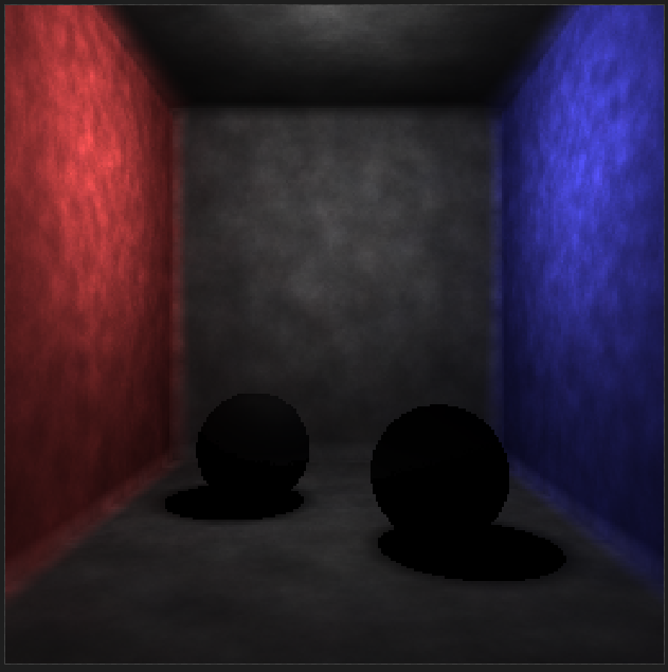
\includegraphics[width=0.5\textwidth]{direct_diffuse}
\caption{Render with direct diffuse lighting only}
\label{fig:direct_diffuse}
\end{figure}

\subsubsection{Specular \& Gloss}
This was straight forward to implement as, due to the intensity, it is rendered using the existing raytracing method that was developed during the lab handins.

\subsubsection{Caustics}
Caustics are computationally intensive to calculate using standard raytracing methods but was straight forward to implement using a seperate caustic photon map. In a caustic map photons are emitted from the light source to reflective and transmissive objects, later when rendering the caustic map is calculated using a radience estimate. A caustic map can be filtered prior to rendering to smooth out hard edges - this hasn't been done in my implementation due to time constraints.
\begin{figure}[h]
\centering
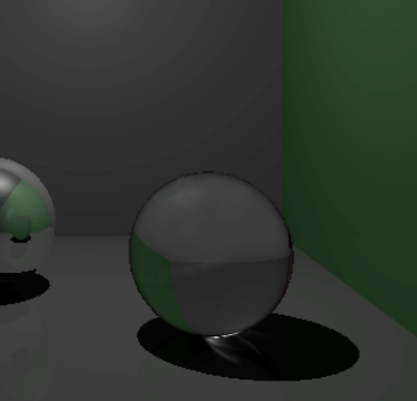
\includegraphics[width=0.5\textwidth]{caustics}
\caption{Render with caustics}
\label{fig:caustics}
\end{figure}

\end{document}
